\documentclass[11pt]{article}
\usepackage{amsmath,textcomp,amssymb,geometry,graphicx,enumerate}

\def\Name{Quoc Thai Nguyen Truong}  % Your name
\def\SID{24547327}  % Your student ID number
\def\Login{cs170-ig} % Your login (your class account, cs170-xy)
\def\Homework{11}%Number of Homework
\def\Session{Fall 2014}

%for code%
\usepackage{listings}
\lstset{language=python}


\title{CS170--Fall 2014 --- Solutions to Homework \Homework}
\author{\Name, SID \SID, \texttt{\Login}}
\markboth{CS170--\Session\  Homework \Homework\ \Name}{CS170--\Session\ Homework \Homework\ \Name, \texttt{\Login}}
\pagestyle{myheadings}

\newenvironment{qparts}{\begin{enumerate}[{(}a{)}]}{\end{enumerate}}
\def\endproofmark{$\Box$}
\newenvironment{proof}{\par{\bf Proof}:}{\endproofmark\smallskip}

\textheight=9in
\textwidth=6.5in
\topmargin=-.75in
\oddsidemargin=0.25in
\evensidemargin=0.25in

\newcommand{\tab}{\hspace*{2em}}

\begin{document}
\maketitle

\noindent
Collaborators: Kiet, Aditya


% Based upon a template file from Ivan Smirnov - thank you Ivan!

\section*{1. Beyond Suspicion}
\begin{qparts}
\item Suspected False
\item True
\item True
\item Suspected False
\item Suspected True
\item True
\item True
\item Suspected False
\end{qparts}

\newpage
\section*{2. Approximation Algorithms}


\textbf{Proof.}\\
Let w be the total weight of the minimum Steiner tree.\\
Let r be the weight in G$^\prime$ that cost to visit every special nodes in S.\\
Let b be the total weight Steiner tree output from the approximation algorithm in the problem.\\
To prove that this algorithm achieves an approximation ratio of 2, we want to show that 
the ratio of $b$ and $w$ to be less than 2 which is $2w \geq b$\\
\\
If we do DFS on the optimal minimum Steiner tree to create a tour ,and traverse all nodes and return to the source, it will give us a total weight of 2w.\\
If we apply the same on graph G$^\prime$, then the total weight would be less than the optimal minimum Steiner tree.\\
The reason is not all the shortest distances between nodes u and v (u,v are in S) exist in graph G. We also remove any duplicate nodes in the tour in graph G$^\prime$. Hence, the weight must be less than 2w.\\
In step 3, we add all edges that is also edges from minimum spanning tree. Hence, weight b can't be greater the weight r. Therefore, $b \leq r \leq 2w$\\
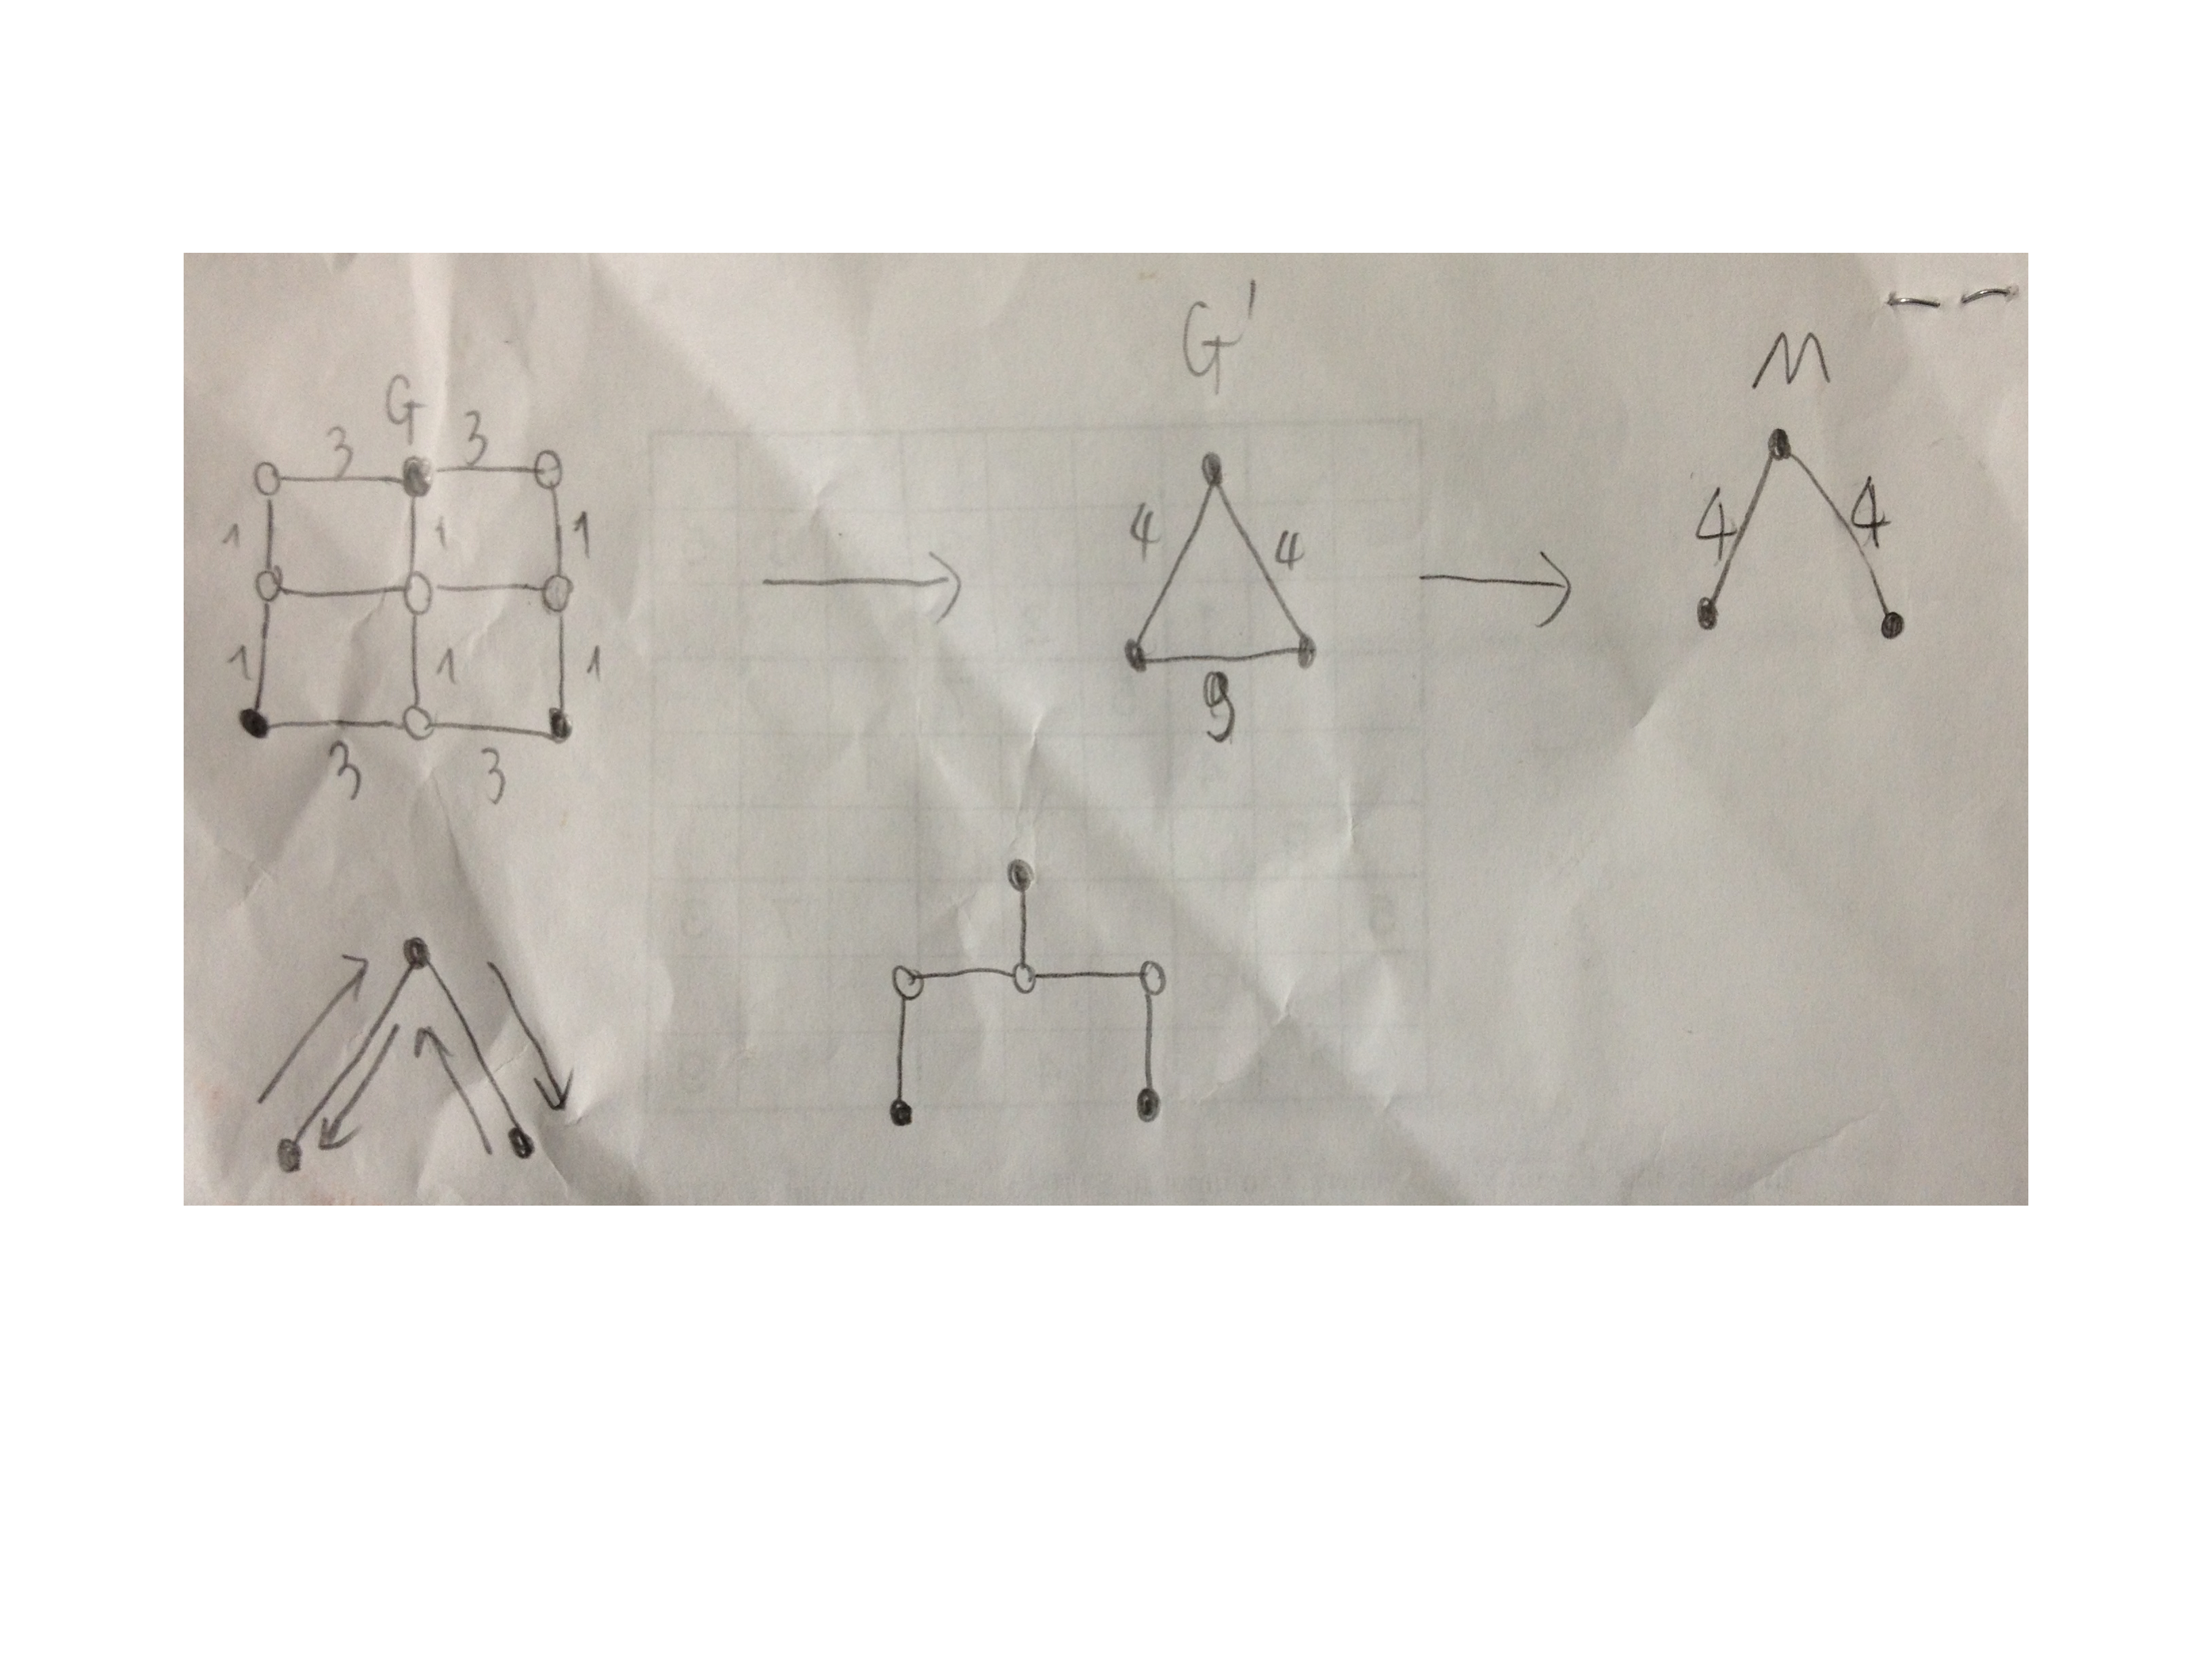
\includegraphics[scale=0.165]{2.PNG}
\newpage
\section*{3. Algorithm Design Practice}

\noindent
\textbf{Main idea.}\\
The idea is to use Dynamic programming with memorization to solve this problem.\\
Let P(i) = largest index j, such that $j < i$ , and interval j does not overlap with interval i, we use binary search in order to find j in the list of $([l_1,r_1], \cdots, [l_i,r_i])$\\
Let B(i) = the optimal solution which is the best weight attainable from non-overlap intervals $([l_1,r_1], \cdots, [l_i,r_i])$\\
There are 2 cases:\\
 + If the weight $w_i$ of the current interval$[l_i,r_i]$ is in the optimal solution, then $B(i) = w_i + B(P[i])$.\\
 + Else : $B(j) = B(i-1)$.\\
In these 2 cases, we pick the one which give the higher total weight between intervals $([l_1,r_1], \cdots, [l_i,r_i])$ that don't overlap.\\
Therefore we have a recurrence relation:
$$B(i) = max(w_i + B(P[i]), B(i-1))$$
\noindent
\textbf{Pseudocode.}\\
Line 0: M = [], M[0] = 0\\
Line 1: P = [], P[0] = 0\\
Line 2: Computer P using  binary search in order to find largest index j value interval that does not overlap in the list for every index i in P\\
Line 3: BestWeigth(($[l_1,r_1], \cdots, [l_k,r_k]$), $(w_1,\cdots, w_k)$):\\
Line 4:\tab If $k == 0$: return 0\\
Line 5:\tab for $i:= 1$ to k:\\
Line 6:\tab\tab $M[i] = max(w_i + M[P[i]], M[i - 1])$\\
Line 7:\tab return M[k]\\

\noindent
\textbf{Proof of correctness.}\\
Looking at the algorithm, we can see that it broke into sub-problems that are getting the maximum weights between non-overlap intervals. In the For loop, each time when it invokes M[i], it will calls $M[P[i]]$ ($P[i] < i$) and $M[i-1]$, and we know for sure that $M[P[i]]$ stores the optimal solution which is the best weight attainable from non-overlap intervals ($[l_1,r_1], \cdots, [l_{P[i]},r_{P[i]}]$), and $M[i-1]$ stores the optimal solution which is the best weight attainable from non-overlap intervals ($[l_1,r_1], \cdots, [l_{i-1},r_{i-1}]$). Hence, we just update a new optimal solution which give the maximum value between $w_i + M[P[i]]$ and $ M[i - 1]$. We can see that the For loop iterate k times, so M[k] is the optimal solution which is the best weight attainable from non-overlap intervals $([l_1,r_1], \cdots, [l_k,r_k])$. Therefore, the algorithm return the best total weight of non-overlap intervals in k intervals.\\

\noindent
\textbf{Running time.}
$$\boxed{T(k)= \Theta(klog(k))}$$ 

\noindent
\textbf{Justification of running time.}\\
Let T(k) be the run time of the algorithm with k intervals (k weights).\\
At line 2: since the list is pre-sorted by the end value, using binary search in order to find largest index for array P take $\Theta(k\log(k)$. Call it k time and each time take $\Theta(\log(k))$\\
At line 5 and 6: each time when it invokes $M[i]$, it calls $M[P[i]]$ ($P[i] < i$) and $M[i-1]$ which we already have, so it take constant time to lookup and find the maximum value. We know that it iterate from 1 to k.\\ 
Therefore, 
$$T(k) = \Theta(klog(k)) + \Theta(k)$$
$$\boxed{T(k) = \Theta(k\log(k))}$$


\newpage
\section*{4. Learn to use a SAT solver}

\noindent
\textbf{Final answer.}\\
$\boxed{Yes}$. Alice could be a werewolf

\noindent
\textbf{List of variables and explanations.}\\
\begin{itemize}
\item Let A be Alice is a knight
\item Let B be Bob is a knight
\item Let C be Carol is a knight
\item Let !A be Alice is a Knave
\item Let !B be Bob is a Knave
\item Let !C be Carol is a Knave
\item Let WA be A is a werewolf
\item Let WB be B is a werewolf
\item Let WC be C is a werewolf
\item Let !WA be A is not a werewolf
\item Let !WB be B is not a werewolf
\end{itemize}

\noindent
\textbf{Listing of STP file.}
\begin{verbatim}
A => WA
!A => !WA 
B => WB
!B => !WB
C => (!A and !B)
!C => (A and B)
\end{verbatim}
STP Input:\\
\includegraphics[scale=1]{in4.PNG}\\
STP OutPut:\\
\includegraphics[scale=1]{out4.PNG}
\newpage
\section*{5. Sudoku}

\noindent
\textbf{Main idea.}
We use 9 variables represent 9 number (1 to 9).\\
We solve this problem by create constraints . So for each of 9 variables, we create all the possible constraints for the row, columns, 3x3 blocks to make sure that number 1 to 9 are unique in each of row, columns, 3x3 blocks constraints.

\noindent
\textbf{Description of boolean variables.}
\begin{itemize}
\item $a11,a12,\cdots, a99 = 1$
\item $b11,b12,\cdots, b99 = 2$
\item $c11,c12,\cdots, c99 = 3$
\item $d11,d12,\cdots, d99 = 4$
\item $e11,e12,\cdots, e99 = 5$
\item $f11,f12,\cdots, f99 = 6$
\item $g11,g12,\cdots, g99 = 7$
\item $h11,h12,\cdots, h99 = 8$
\item $i11,i12,\cdots, i99 = 9$
\end{itemize}

\noindent
\textbf{Solution to Sudoku puzzle.}

% Replace the x's below with your solution
% (Or show your solution in some other way, that's fine too.)
\begin{tabular}{||c|c|c||c|c|c||c|c|c||}
\hline
\hline
9&8&7 &6&5&4 &3&2&1\\
\hline
2&4&6 &1&7&3 &9&8&5\\
\hline
3&5&1 &9&2&8 &7&4&6\\
\hline
\hline
1&2&8 &5&3&7 &6&9&4\\
\hline
6&3&4 &8&9&2 &1&5&7\\
\hline
7&9&5 &4&6&1 &8&3&2\\
\hline
\hline
5&1&9 &2&8&6 &4&7&3\\
\hline
4&7&2 &3&1&9 &5&6&8\\
\hline
8&6&3 &7&4&5 &2&1&9\\
\hline
\hline
\end{tabular}
\bigskip

\noindent
\textbf{Program used to generate input to STP.}\\
PLEASE LOOK AT NEXT PAGE \\
\includegraphics[scale=0.46]{5_1.PNG}\\
\includegraphics[scale=0.5]{5_2.PNG}



\end{document}
